% !TeX program = lualatex

\documentclass[12pt]{article}



\usepackage[margin=1in]{geometry} 
\usepackage{amsmath,amsthm,amssymb}
\usepackage{MnSymbol}
\usepackage{graphicx}
\usepackage{bm}
\usepackage[normalem,normalbf]{ulem}
\usepackage{algorithm} 
\usepackage{algpseudocode} 
\usepackage{multirow}
\usepackage{rotating}
\usepackage{therefore}

\usepackage{tikz}
\usetikzlibrary{shapes.multipart}
\usetikzlibrary{shapes.symbols}

\usetikzlibrary{graphs,graphdrawing,graphs.standard,quotes}
\usegdlibrary{circular,force,layered,routing}
\tikzset{
	graphs/simpleer/.style={
		nodes={draw,circle, blue, left color=blue!20, text=black, inner sep=1pt},
		node distance=2.5cm, nodes={minimum size=2em}
	},
	every loop/.style={},
}

\newcommand*\circled[1]{\tikz[baseline=(char.base)]{
		\node[shape=circle,draw,inner sep=2pt] (char) {#1};}}

\newcommand{\m}{\medskip\\}
\newcommand{\N}{\mathbb{N}}
\newcommand{\Z}{\mathbb{Z}}
\newcommand{\R}{\mathbb{R}}
\newcommand{\bbs}{\textbackslash\textbackslash\space}
\newcommand{\bs}{\textbackslash\space}
\newcommand{\la}{\enskip\land\enskip}
\newcommand{\lo}{\enskip\lor\enskip}
\newcommand{\comp}[1]{#1^\mathsf{c}}
\newcommand{\micdrop}{\qed}
\newcommand{\contra}{\begin{tikzpicture}
		\node[starburst, draw, minimum width=3cm, minimum height=2cm,line width=1.5pt,red,fill=yellow,scale=.5]
		{BOOM, A CONTRADICTION!!!};
\end{tikzpicture}}

\renewcommand{\qedsymbol}{$\blacksquare$}

\DeclareMathOperator{\lcm}{lcm}

\newtheorem{theorem}{Theorem}

\newenvironment{exercise}[2][Exercise]{\begin{trivlist}
		\item[\hskip \labelsep {\bfseries #1}\hskip \labelsep {\bfseries #2.}]}{\end{trivlist}}

\setlength\parindent{24pt}

\makeatletter
\renewcommand*\env@matrix[1][*\c@MaxMatrixCols c]{%
	\hskip -\arraycolsep
	\let\@ifnextchar\new@ifnextchar
	\array{#1}}
\makeatother
\setlength\parindent{24pt}


\begin{document}
	
	% --------------------------------------------------------------
	%                         Start here
	% --------------------------------------------------------------
	
	
	\title{Homework 7 (Due March 15, 2023)}
	\author{Jack Hyatt\\ %replace with your name
		MATH 575 - Discrete Mathematics II - Spring 2023} 
	
	\maketitle
	
	Justify all of your answers completely.\\
	
	
	\medskip 
	
	\begin{enumerate}

\item Let $k \geq 2$. Suppose $G$ is a $k$-connected graph with at least $k+1$ vertices, and let $S \subseteq V(G)$ with $|S| = k$. Prove that for every pair of vertices $x,y \in S$, there exists a cycle in $G$ containing $x$ and $y$ that avoids $S - \{x,y\}$.
\begin{proof}
	Let $k \geq 2$. Suppose $G$ is a $k$-connected graph with at least $k+1$ vertices, and let $S \subseteq V(G)$ with $|S| = k$. Let $x,y \in S$. Since $G$ is $k$-connected, there are $k$ disjoint $x,y$-paths in $G$. At most, $k-2$ paths can contain a vertex in $S$, since $|S-{x,y}|$ is $k-2$. So then we have two disjoint $x,y$-paths avoiding $S-{x,y}$. Combining those two paths will give the desired cycle. 
\end{proof}

\medskip 

\item Use Menger's Theorem ($\kappa(x,y) = \lambda(x,y)$ for all nonadjacent $x,y$) to prove the K\"onig--Egerv\'ary Theorem (if $G$ is bipartite, then $\beta(G) = \alpha'(G)$).\m
$\beta(G)$ is size of minimum vertex cover of G.\\
$\alpha'(G)$ is size of a maximum matching in G\\
$\kappa(x,y)$ is min size of an x,y-separator.\\
$\lambda(x,y)$ is max number of pairwise internally disjoint x,y-paths.
\begin{proof}
	Assume $G = X \cupdot Y$ is bipartite with bipartitions $X$ and $Y$. One would have to be a toddler to not see that $\alpha'(G)\leq\beta(G)$. So it is sufficient enough for me to show that $\alpha'(G)\geq\beta(G)$.\\
%	\textbf{Case 1}: There is no pair of vertices between $X$ and $Y$ that doesn't have an edge. Then $G$ is a complete bipartite graph.\\
%	WLOG, let $|X|\leq|Y|$. Since $G$ is $K_{|X|,|Y|}$, Hall's Theorem lets us know that $\alpha'(G) = |X|$. Since $G$ is complete, a minimum vertex cover is just the smaller biparitition, namely $X$. So then $\beta(G) = |X| = \alpha'(G)$.\\
%	\textbf{Case 2}: There exists at least one pair of vertices, one in $X$ and one in $Y$, that are not adjacent.
	Let us stick a source vertex, $s$, to be adjacent to all of $X$ and a sink vertex, $t$, to be adjacent to all of $Y$. We shall name this new graph $G'$. If we consider a minimum $s,t$-separator, we see the set is also a vertex cover of $G$ since if it wasn't, we would have an edge between $X$ and $Y$ which gives us an $s,t$-path. So then a minimum vertex cover would be at most that. So then $\beta(G)\leq\kappa(s,t)$.\\
	Let us consider the maximum set of pairwise internally disjoint $s,t$-paths. Each path uses different vertices in $X$ and $Y$. So then the edges from $X$ to $Y$ in those paths will create a matching. So then a maximum matching would be at least that. So then $\lambda(s,t)\leq\alpha(G)$.
	Then by Menger's Theorem, we get $\beta(G)\leq\kappa(s,t) = \lambda(s,t)\leq\alpha(G)$. So $\beta(G)\leq\alpha(G)$.
\end{proof}


\medskip
\item Let $D$ be an $s,t$-network with no directed path from $s$ to $t$. Prove that $D$ cannot have a feasible flow with value greater than 0. 
\begin{proof}
	Let $D$ be an $s,t$-network with no directed path from $s$ to $t$. Then there exists an $S,T$-cut with no edges going from $S$ to $T$; where $s\in S$, $t\in T$, and $S$ and $T$ partition $D$. This is true since if every $S,T$-cut had at least one edge going from $S$ to $T$, we'd be able to construct a directed path from $s$ to $t$.\\
	So there exists a $S,T$-cut with flow 0. By weak duality, this means the value of the flow is less than or equal to 0.
\end{proof}

\medskip 

\item Consider the following $s,t$-network with flow $f$.
\begin{center}
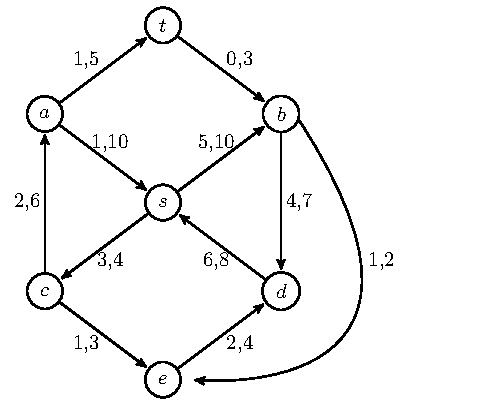
\includegraphics[scale=1]{7_1.pdf}
\end{center}
\begin{enumerate}
\item Verify that $f$ is feasible.\m
$f$ is not feasible since $t$ does not follow the conservation of flow. The argument that we don't consider the source and sink in that law is flawed, since there are edges coming into $s$ and out of $t$. We don't consider the source and sink when they only have edges going in the source and out of the sink. When they have both kinds of edges, we include them in the law. So I am putting and foot down and will not pretend $t$ doesn't make $f$ infeasible. Same also about $s$. I know you agree with me Kaylee.
\item Use the Ford-Fulkerson algorithm to find a maximum flow of the network. Prove that your final flow is maximum by constructing a minimum cut. \m
Ford and Fulkerson both descend from the heavens and sat on my shoulders like devils, and used their silver tongues to convince me to \emph{GREEDILY} make me take the $s,c,a,t$ path, filling each edge up to 4. I then look to the heavens as I fall to my knees, knowing that I will never be able to increase this flow anymore, as a vision of an $S,T$-cut of value 4 came upon me. As I close my eyes, I recite the set $S=\{s,e,d,b\}$. As I open my eyes, I ponder to myself what edges go from $S$ to $T$, the set containing the other vertices I did not proclaim. The epiphany appeared in my head that there is only one edge to do so, namely $sc$, which has a value of 4. The nightmare has now passed, and so I lay unmoving, appalled by how low the value of my flow is. I cry...
\end{enumerate}

\medskip 
\item A warehouse stores 3 different chemicals A, B, and C. Tomorrow, 4 trucks will arrive to transport the barrels of chemicals to another location. Due to safety concerns there are some restrictions for their transportation.
\begin{enumerate}
\item[i.] Chemical A can only be transported in Truck \#1 or Truck \#2. No truck can carry more than 2 barrels of Chemical A. 
\item[ii.] Chemical B can only be transported in Truck \#2 or Truck \#3. No truck can carry more than 2 barrels of Chemical B. 
\item[iii.] Chemical C can be transported in any truck, but no truck can carry more than 1 barrel of Chemical C. 
\end{enumerate}

Moreover, each truck has their own carrying capacity: Truck \#1 can carry at most 3 total barrels; Truck \#2 can carry at most 4 total barrrels; Truck \#3 can carry at most at most 7 total barrels; and Truck \#4 can carry at most 3 total barrels. Suppose the warehouse currently has 4 barrels of each chemical in storage (12 total barrels). 

Find the maximum total number of barrels that can be shipped using the 4 trucks. Verify that your answer is maximum.\m

%\begin{center}
%	\tikz \graph[grow=right, branch down=2cm, edge quotes=above, left anchor=east] {
%		s [yshift=-1cm] -> {A,B,C} -!-  {[nodes = {xshift = 1cm}] 1,2,3,4} -> 
%		t [yshift=-1cm, xshift=1cm];
%		A -> ["0,2"] 1;
%		A -> ["0,2"] 2;
%		B -> ["0,2"] 2;
%		B -> ["0,2"]3;
%		C -> ["0,1"] {1,2,3,4};
%	};
%\end{center}

I am furious. I tried my darnedest to get the tikz graph package to draw this out, but the labeling of the edges kept getting in the way of each other. So this is my bad drawing of it on my iPad >:(
\begin{center}
	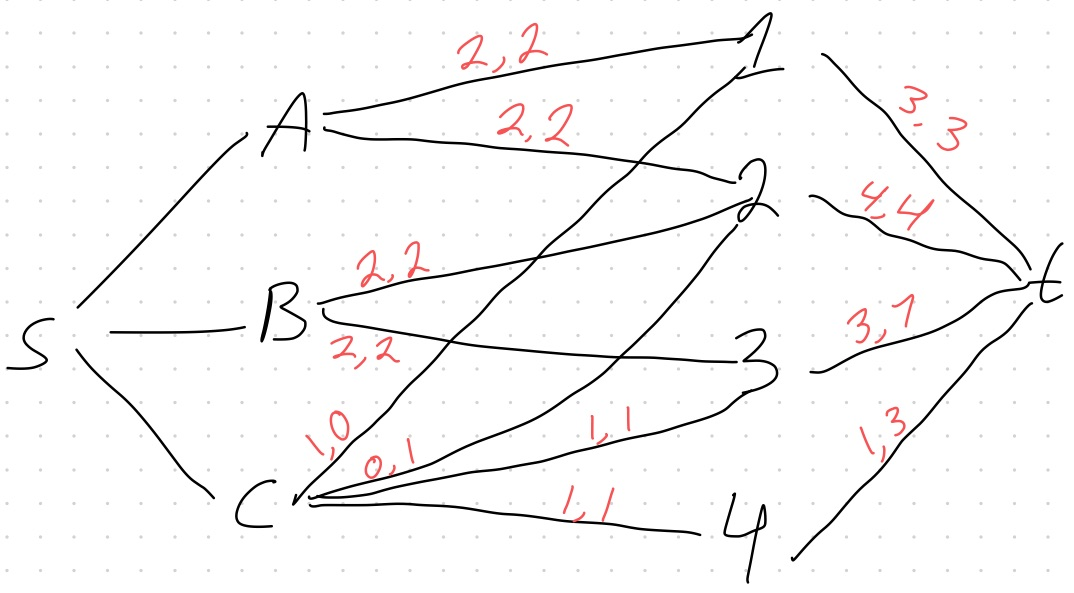
\includegraphics[scale=0.75]{7_5.png}
\end{center}
This flow gives a value of 11, which I know is maximum since I can find a $S,T$-cut of the same value. Let $S=\{s,A,B,C,1,2\}$ and $T=G-S$. The cut is $\{1t,2t,B3,C3,C4\}$.

\end{enumerate}
\end{document}
